\section{\acf{tool}}\label{sec:toolbox}
% This chapter describes the top-level architecture of the 
\todo[inline]{short description of the chapter}
\todo[inline]{something about the Simulink Add-Ons that are used by the toolbox}
\todo[inline]{describe briefly what is the input and the output of the whole toolbox}

\subsection{Objectives}\label{toolbox:objectives}


\subsection{Architecture}
    \ac{tool} is divided into two parts: 1) Parts Library and 2) Modular Simulation. The Parts Library contains Simulink subsystems, which can be connected to form simulations of various complexity and for multiple scenarios. The other is a Modular Simulation, which can be set up with either MATLAB command line scripts or graphical user interface.

    \subsubsection{Parts Library}
        %TODO: Should I write something about the aim of the library?
        \ac{scars} Parts Library is a ready to use Simulink Custom Library, that is a collection of blocks available to use in Simulink models. All blocks in library downloaded alongside \ac{scars} are parametrized, masked and described to ease the integration of library parts into user simulation. The library is divided into specific sections:
        \begin{itemize}
            \item Satellite Dynamics
            \item Reference Frames Transformations
            \item Environment
            \item Actuators
            \item Sensors
            \item Control Algorithms
            \item Visualization
            \item Analysis
            \item Examples
        \end{itemize}

        \begin{figure}[H]
            \centering
            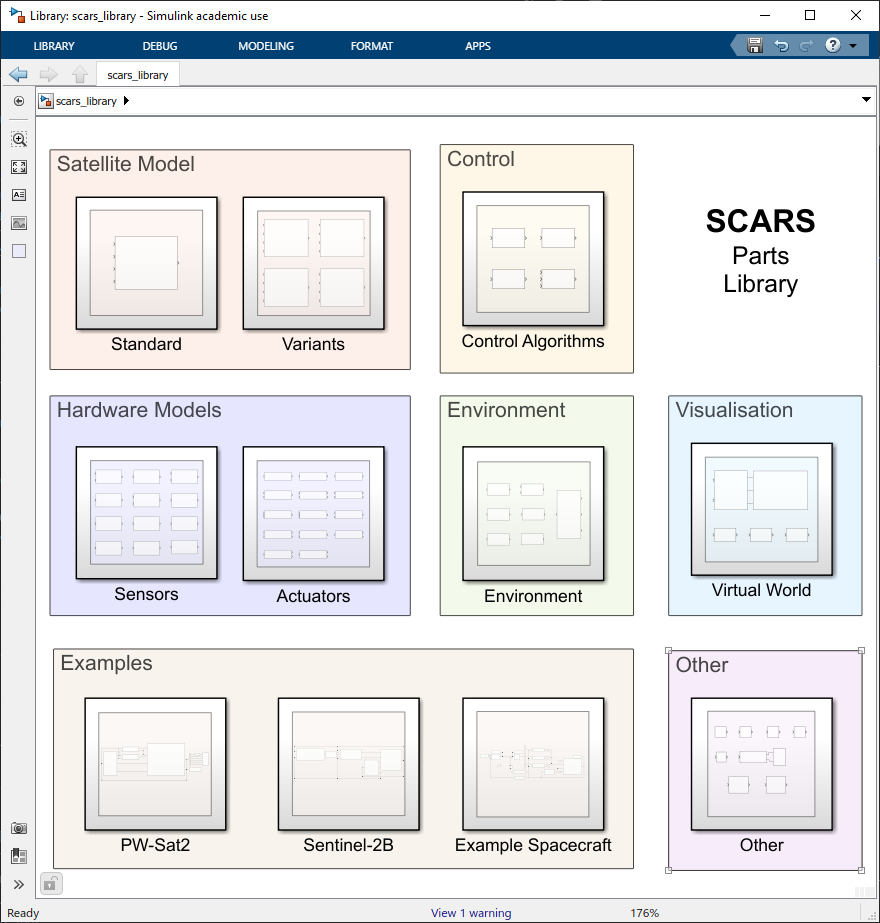
\includegraphics[width=1\textwidth]{2-toolbox/scars-library.png}
            \caption{SCARS Parts Library screenshot}
            \label{fig:scars-library}
        \end{figure}

    \subsubsection{Modular Simulation}
        \ac{scars} Modular Simulation is a ready-made simulink model available for setup using prepared scripts and \ac{scars} user interface. The model is a simulation of cube-shaped satellite, which can be set on specified orbit using various initialization methods, such as Keplerian elements in conjunction with Julian date time. (The initialization is further described in Chapter \ref{sec:documentation}). In the same manner, all actuators and sensors available in \ac{scars} library can be chosen. The Modular Simulation makes use of most available blocks, which can be commented out from the model, either by hand or using the user interface, to improve the speed of the simulation.

        \begin{figure}[H]
            \centering
            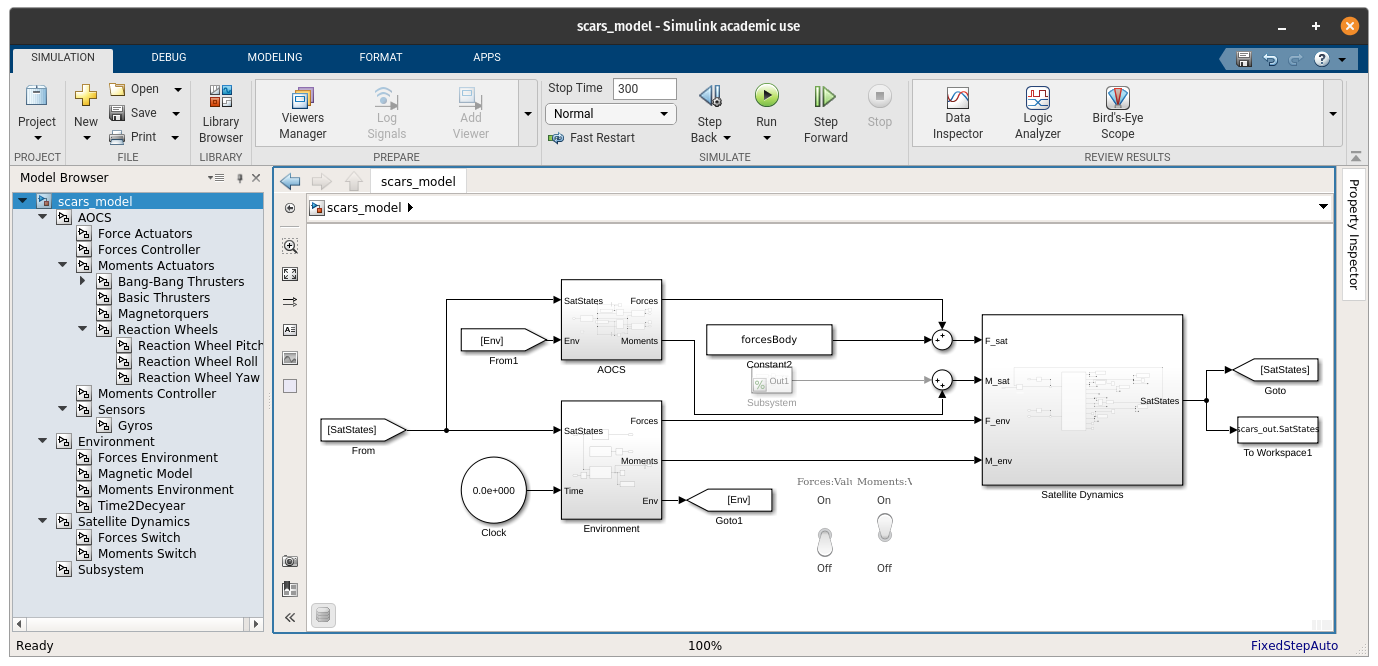
\includegraphics[width=1\textwidth]{2-toolbox/scars-model.png}
            \caption{SCARS Modular Simulation screenshot}
            \label{fig:scars-model}
        \end{figure}
